\chapter{Neutrino Masses}
\section{Neutrino Oscillations}
\subsection{Evidence and Motivation}
It is based on the observation that neutrinos disappear, or change flavour between source and detector!

\paragraph{Solar neutrinos} are produced by following mechanisms (all $\beta$-decays!)
\begin{itemize}
   \item $pp$-neutrinos: produced by $4p \rightarrow {}^4 \text{He} + 2 e^+ + 2 \nu_e$; $E_{\nu_e} < \SI{0.42}{\mega \eV}$; flux $\phi= \SI{6e10}{\cm\tothe{-2}\s\tothe{-1}}$
   \item $pep$-neutrinos: produced by $p+e^-+p \rightarrow d + \nu_e$; $E_{\nu_e} < \SI{1.44}{\mega \eV}$; flux $\phi=\SI{0.015e10}{\cm\tothe{-2}\s\tothe{-1}}$
   \item $Be$-neutrinos: produced by ${}^{7}\text{Be} + e^- \rightarrow {}^7 Li + \nu_e$; $E_{\nu_e} < \SI{0.86}{\mega \eV}$; flux $\phi=\SI{0.48e10}{\cm\tothe{-2}\s\tothe{-1}}$
   \item $B$-neutrinos: produced by ${}^8 \text{B} \rightarrow {}^8 \text{Be} + e^+ + \nu_e$; $E_{\nu_e} = \SI{14}{\mega \eV}$; flux $\phi=\SI{0.5e7}{\cm\tothe{-2}\s\tothe{-1}}$
\end{itemize}
Note that only electron neutrinos are produced!

\begin{figure}[htpb]
   \centering
   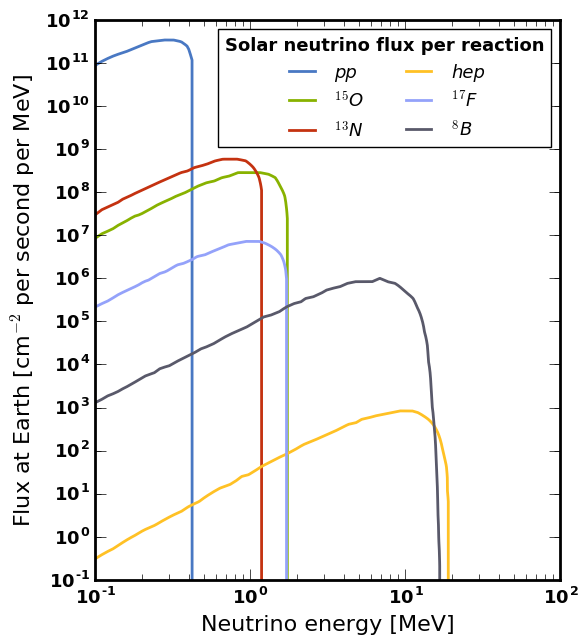
\includegraphics[width=0.5\linewidth]{Solar_neutrino_flux_spectrum.png}
   \caption{Solar neutrino flux spectrum\cite{wiki:solarNu}}%
   \label{fig:}
\end{figure}

Detection of neutrinos can be achieved by
\begin{itemize}
   \item Chemical via $(A,Z) + \nu_e \rightarrow (A,Z+1) + e^-$. Extract new element using chemistry and observe its decay. Used for Cl and Ga targets.
   \item Reverse electron capture $\nu_e + n \rightarrow e^- + p $. Detect $e^-$ in Cherenkov scintillation detection.
   \item Elastic scattering off electron $\nu + e^- \rightarrow \nu + e^-$. Detect scattered $e^-$, and mostly used for $\nu_e$ (CC-contribution).
   \item Scattering off deuterium $\nu + d \rightarrow \nu + n + p$. Detect free neutron. Here all neutrinos contribute equally. 
\end{itemize}

Results are
\begin{itemize}
   \item Between $1/3$ and $2/3$ of produced in the Sun (known from Solar energy output and solar modelling) do not participate in CC reactions ("disappear").
   \item Total active neutrino flux measured at Sudbury Neutrino Observatory (SNO) does agree with predictions.
\end{itemize}
So we conclude $\nu_e \rightarrow \nu_\mu, \nu_\tau$.

\paragraph{Atmospheric neutrinos} are produced by hardonic shower from cosmic rays hitting atmosphere. 
\begin{align}
   \pi^\pm &\rightarrow \mu^\pm + \nu_\mu (\bar{\nu}_\mu) \\
   \mu^\pm &\rightarrow e^\pm + \nu_e(\bar{\nu}_e) + \nu_\mu(\bar{\nu}_\mu)
\end{align}
We expect two $\nu_\mu (\bar{\nu}_\mu)$ for each $\nu_e (\bar{\nu}_e)$ at $E \lessapprox \SI{10}{\giga \eV}$. But roughly equal numbers of $\nu_e$ and $\nu_\mu$ are observed via $\nu_l + N \rightarrow l + X$ with $l=e,\mu$. The interpretation is that mostly $\nu_\mu (\bar{\nu}_\mu) \rightarrow \nu_e (\bar{\nu}_e)$.

\paragraph{Reactor neutrinos} are produced by nuclear fission where the remnants are unstable because of "too many neutrons"
\begin{align}
   (A,Z) \rightarrow (A, Z+1) + e^- + \bar{\nu}_e 
\end{align}
And $E_{\bar{\nu}_e} \sim \si{\mega \eV}$. Its detection is done by scintillation detectors $\bar{\nu}_e + p \rightarrow e^+ + n$. KAMLand experiment found significant deficit of $\bar{\nu}_e$ at $L \sim \SI{100}{\kilo \m}$. At Daya Bay and Reno experiments, it is found few percent deficit at $L\sim \SI{1}{\kilo\m}$.

\paragraph{Neutrino beams} are produced by meson beam decay. Mostly $\nu_\mu (\bar{\nu}_\mu)$ from $\pi^\pm$ decay. However, there is some contamination of $\nub{e}$, also from Kaon decay $K^\pm \rightarrow \pi^0 e^\pm \nub{e} $. K2K experiment (Japan) and MINOS experiment (USA) find significant deficits at $L\sim \SI{100}{\kilo\m}$ and $E_\mu \sim \SI{1}{\giga \eV}$. Interpretation is mostly $\nu_\mu \rightarrow \nu_\tau$.

All together the most likely interpretation is neutrino flavor oscillations!

\subsection{Theory}
Suppose that neutrinos have non-trivial mass matrix, as quarks do. Their mass eigenstates $v_i$ are linear combinations of flavour eigenstates $\nu_\alpha$
\begin{align}
   \nu_\alpha &= \sum_{j} U_{\alpha j} \nu_j, \label{1.1} \\
   \nu_i &= \sum_{\alpha} U^*_{\alpha j} \nu_\alpha.
\end{align}
Obviously $U$ is unitary matrix
\begin{align*}
   \sum_{j} U_{\alpha j} U^*_{\beta j} = \delta_{\alpha \beta}, \quad
   \sum_{\alpha} U_{\alpha j} U^*_{\alpha k} = \delta_{jk}.
\end{align*}

Flavour is defined by gauge i.a., in particular by CC interactions of charged leptons. CC interactions vertex involves $e$ and $\nu_e$ as well.

For stable neutrinos, the mass eigenstates are orthonormal
\begin{align}
   \braket{ \nu_i (t) | \nu_j (t)} = \delta_{ij}.
\end{align}
Representing the mass eigenstates in terms of flavour eigenstates with equation (\ref{1.1})
\begin{align}
   \sum_{\alpha, \beta} U^*_{\alpha j} U_{\beta i} \braket{\nu_\beta (t) | \nu_\alpha (t)} &= \delta_{ij}, \notag \\
   \sum_{\alpha, \beta, i, j} U^*_{\alpha j} U_{\gamma j} U_{\beta i} U^*_{\delta i} \braket{\nu_\beta (t ) | \nu_\alpha (t)} &= \sum_{i,j} \delta_{ij} U_{\gamma j} U^*_{\delta i}, \notag \\
   \sum_{\alpha, \beta, i, j} \delta_{\alpha \gamma} \delta_{\beta \delta} \braket{\nu_\beta(t) | \nu_\alpha(t)} &= \sum_{i} U_{\gamma i} U^*_{\delta i} = \delta_{\gamma \delta}. \label{1.3}
\end{align}
On the second line, $\sum U_{\gamma j} U^*_{\delta i}$ is multiplied to both sides. Flavour states are also orthonormal!

\paragraph{Flavour transition amplitudes} using plane waves (QM treatment). Produce flavour $\alpha$ at $\pmb{x} = 0$ and $t=0$. We want to find out amplitude for transition to flavour $\beta$ at $\pmb{x}, t$.
\begin{align}
   A_{\alpha \rightarrow \beta} (t, \pmb{x}) &= \braket{\nu_\beta (t,\pmb{x}) | \nu_\alpha(0)} \\
                                             &= \braket{\nu_\beta (0)| \exp[-i(\hat{H}_\text{free} t - \hat{\pmb{p}} \cdot \pmb{x})] | \nu_\alpha (0)} \notag
\end{align}
Since $\nu_\alpha$ is not mass eigenstate, it is not eigenstate of $\hat{H}_\text{free}$ either. Remember in QM, $\hat{p}\psi = -i \partial_x \psi$. Use equation (\ref{1.1}) and assume plane wave (momentum eigenstate) in second step
\begin{align}
   A_{\alpha \rightarrow \beta } (t, \pmb{x}) &= \sum_{j} \braket{\nu_\beta (0)| \exp[-i(\hat{H}_\text{free} t - \hat{\pmb{p}} \cdot \pmb{x})] U_{\alpha j}| \nu_j (0)} \notag \\
                                              &= \sum_{j} \braket{\nu_\beta (0)|U_{\alpha j} \exp[-i(E_j t - \pmb{p}_j \cdot \pmb{x})] | \nu_j (0)} \notag \\
                                              &\stackrel{(\ref{1.1})}{=} \sum_{j,\gamma} \braket{\nu_\beta(0) | U_{\alpha j} \exp[-i(E_j t - \pmb{p}_j \cdot \pmb{x})] U^*_{\gamma j} | \nu_\gamma (0)} \notag \\
                                              &\stackrel{(\ref{1.3})}{=} \sum_j U_{\alpha j} U^*_{\beta j} \exp[-i(E_j t - \pmb{p}_j \cdot \pmb{x})] \label{1.6}
\end{align}

The transition probability
\begin{align}
   P_{\alpha \rightarrow \beta}(t, \pmb{x}) &= \left| A_{\alpha \rightarrow \beta} (t, \pmb{x}) \right|^2, \notag \\
                                            & = \sum_{k,j} U_{\alpha j} U^*_{\beta j} \exp[-i(E_j t - \pmb{p}_j \cdot \pmb{x})] U_{\alpha k} U^*_{\beta k} \exp[i(E_k t - \pmb{p}_k \cdot \pmb{x})] \notag \\
                                            &= \sum_{k,j} U_{\alpha j} U^*_{\alpha k} U_{\beta k} U^*_{\beta j} \exp[-i((E_j - E_k) t - (\pmb{p}_j - \pmb{p}_k) \cdot \pmb{x})] \label{1.7}
\end{align}
Note that off-diagonal ($k\neq j$) contributions have non-trivial phase factor and it leads to oscillations!

\paragraph{Example} with 2 states. The transformation matrix can easily be parametrized by a rotation $\theta$
\begin{align}
   U = U^* = \begin{pmatrix} \cos(\theta) & \sin (\theta) \\ -\sin (\theta) & \cos (\theta) \end{pmatrix} \label{1.8}
\end{align}
Then the probability is
\begin{align}
   P_{1\rightarrow 2} &= \cos^2(\theta) \sin^2(\theta) + \sin^2(\theta) \cos^2(\theta) - \sin^2(\theta) \cos^2(\theta)  \exp[-i((E_2 - E_1) t - (\pmb{p}_2 - \pmb{p}_1) \cdot \pmb{x})], \notag \\
                      &\quad - \sin^2(\theta) \cos^2(\theta) \exp[-i((E_1 - E_2) t - (\pmb{p}_1 - \pmb{p}_2) \cdot \pmb{x})], \notag \\
                      &= \cos^2(\theta) \sin^2(\theta) \left[ 2 - 2 \cos((E_2 - E_1)t - (\pmb{p}_2 - \pmb{p}_1)\cdot \pmb{x}) \right], \notag \\
                      &= \sin^2(2\theta) \sin^2[((E_2 - E_1)t - (\pmb{p}_2 - \pmb{p}_1)\cdot \pmb{x})/2]. \label{1.9}
\end{align}
Note  that one needs non-trivial mixing angle ($\theta \neq 0, \pi/2$) and non-zero mass difference for oscillations! To see the latter, expand phase around average momentum $\pmb{p}$ and assume $E \gg m $ (ultra-relativistic limit, reasonable for neutrinos!). Treat the problem in $1$-dimension
\begin{align*}
   E_1 &= \sqrt{m_1^2 + \pmb{p}_1^2}, \\
       &= \sqrt{m_1^2 + p^2 + 2p(p_1 - p) + (p_1 - p)^2}, \\
       &= \frac{m_1^2}{2p} + p  + (p_1 - p) + \order{(p_1-p)^2},
\end{align*} 
\begin{align}
   P_{1\rightarrow 2} = \sin^2(2\theta) \cdot \sin^2 \left[\frac{m_1^2 - m_2^2}{4p}t + (t-x) \frac{p_1-p_2}{2} \right] \label{1.10}
\end{align}
Note
\begin{itemize}
   \item Assumed $t_1 = t_2$ exactly
   \item standard treatment also assumes $t=x$, i.e. classical propagation, or $p_1 = p_2$ (which $E_1 \neq E_2$, since mass eigenstates must be on-shell!)
\end{itemize}

\begin{align}
   P_{1\rightarrow 2} = \sin^2(2\theta) \cdot \sin^2 \left( \frac{\pi x}{L_\text{osc}} \right), \label{1.11}
\end{align}
with oscillation length
\begin{align*}
   L_\text{osc} = \frac{4\pi p}{ \left| m_1^2 - m_2^2 \right| } \approx \frac{4\pi E}{ \left| m_1^2 - m_2^2 \right| }.
\end{align*}
We observe that one needs smaller $E$ to probe smaller $\delta m^2$ at fixed $x$. For more than two states, the expression is similar 
\begin{align}
   L_{ij, \text{osc}} = \frac{4\pi E}{ \left| m_i^2 - m_j^2 \right| }. \label{1.13}
\end{align}

Oscillations have been seen in atmospheric neutrinos! (SuperK, $\sim 1998$) The result can further corrected by QFT\cite{Beuthe_2003}. Phenomenological aspect can be found in \cite{Esteban_2019}. We need two large mixing angles, one small but non-zero. There is probably non-trivial CP-violation.
\begin{align*}
   \Delta m^2_{21} &= (\num{7.4 +- 0.2}) \cdot 10^{-5} \si{\eV \tothe{2}} \\
   \Delta m^2_{31} &= (\num{2.52 +- 0.03})\cdot 10^{-3}\si{\eV \tothe{2}}
\end{align*}
From cosmology, we know $\sum_j m_{\nu_j} \lessapprox \SI{0.5}{\eV}$. So the heaviest neutrino  $m_{\nu_3} \in [\SI{0.04}{\eV}, \SI{0.2}{\eV}] $, much smaller than $m_e$!

\section{Generation of Small Neutrino Masses}
\paragraph{Simplest way}
conceptually is to treat $\nu$'s like charged fermions and introduce $\SU(2)$ singlet right-handed neutrino.
\begin{align}
   \lag_{\text{Yuk}} \supset - \sum_{j,k=1}^{3} \left[ f^{(l)}_{jk} \overline{e^-}_{jR} \phi^\dagger L_{k L} - f^{(\nu)}_{jk} \textcolor{blue}{\bar{\nu}_{jR}} \phi L_{kL} \right] + h.c. \label{1.36}
\end{align}
The resulted mass matrix $(M_l)_{jk}f_{jk}^{(l)} v$ is in general not diagonal. So we need matrix $U_{L,R}$ to diagonalize it
\begin{align}
   l_R^{(p)} = U_R^{(l)}l_R; \quad l_L^{(p)} = U_L^{(l)}l_L  \notag \\
   \overline{l}_R M_l l_L = \overline{l}^{(p)}_R U^{(l)}_R M_l U^{(l)\dagger}_L l_L^{(p)} \label{1.37}
\end{align}

Also transforms $\nu$ in Yukawa terms
\begin{align}
   \lag_{\nu-\text{Yukawa}} = \overline{\nu}_R f^{(\nu)} U_L^{(P)\dagger} \phi L_L.
\end{align}
It gives Dirac mass term; $\nu_R$ is SM singlet ("sterile" neutrino).

To diagonalize $\nu$ mass matrix
\begin{align}
   \nu_R^{(p)} = U_R^{(\nu)} \nu_R, \quad \nu_L^{(p)} = U_L^{(\nu)} U_L^{(e)\dagger}\nu_L
\end{align}

Only $\nu_L$ have gauge so we can only probe 
\begin{align}
   U_{MNS} = \left[ U_L^{(\nu)} U_L^{(l)\dagger} \right]^\dagger = U_L^{(l)} U_L^{(\nu)\dagger}
\end{align}
It is completely analogous to KM matrix in SM.

Drawback is that this mechanism cannot explain $m_{\nu_i} < \SI{1}{\eV}$ with Higgs VEV $v =\SI{175}{\giga\eV}$ and we need $|f^{(\nu)}| < \num{1e-11}$! C.f. to known Yukawas: $f_e \sim \num{3e-6}$, \dots, $f_\tau \approx 1$. So why are $f^{(\nu)}$ so tiny?

\paragraph{Most economical scheme} is via Majorana masses for $\nu_L$ and no sterile neutrinos $\nu_R$!
\begin{align}
   \lag_{\nu-\text{mass}} &= -\frac{1}{2} \sum_{j,k=1}^3 \overline{L^C_{Lj}} \phi \frac{\kappa_{jk}}{M} L_{Lk} \phi  \label{1.41} \\
                          & \stackrel{\phi\rightarrow v}{\longrightarrow} - \frac{v^2}{2M} \sum  \overline{\nu^C_{Lj}} \kappa_{jk} \nu_{Lk} \notag 
\end{align}
Here $L_L \phi$ is $\SU(2) \times \Uni(1)_\text{Y}$ invariant ($Y(\phi)=+1$ and $Y(L)=-1$).
Charge conjugate antiparticle is right-handed field with hypercharge $+\frac{1}{2}$
\begin{align}
   L_L^C = C \overline{L_L}^T.
\end{align}

Charge conjugation matrix $C$ satisfies
\begin{subequations}
   \label{1.42}
\begin{align}
   C^\dagger &= C^{-1}, \label{1.42a}\\
   C^T &= -C,  \label{1.42b}\\
   C \Gamma^T C^{-1} &= \eta_\Gamma \Gamma \label{1.42c},
\end{align}
\end{subequations}
with $\eta_\Gamma = +1 $ for $\Gamma \in \{\id, \gamma_5, \gamma_\mu \gamma_5\}$ and $\eta_\Gamma = -1$ for $\Gamma \in \{\gamma_\mu, \sigma_{\mu\nu}\}$.

Neutrino mass term in equation (\ref{1.41}) does not require new field, but is not renormalizable, since field operators have mass dimension $5$. So in order to keep $\kappa_{jk}$ dimensionless, $1/M$ is needed.

Majorana masses are
\begin{align}
   (m_\nu)_{jk} = \kappa_{jk} v^2 / M . \label{1.43}
\end{align}
Only know large mass scale is (reduced) Planck scale $M_p \simeq \SI{2.4e18}{\giga \eV}$ with $|\kappa_{jk}| \sim \order{1}$. Then $m_{\nu_i} \sim \SI{1e-5}{\eV}$ too small! Need new scale below Planck scale $M \sim \num{1e11} \cdots \SI{1e14}{\giga \eV}$.

Dirac mass term in equation (\ref{1.36}) violates in general lepton favour, but total lepton number is conserved! Hence it allows 
\begin{align}
   \begin{split}
      \mu^- &\rightarrow e^- + \gamma  \\
      \mu^- &\rightarrow e^- + e^+ + e^-
   \end{split} \label{1.44}
\end{align}
But it forbids $0\nu \beta \beta$-decay
\begin{align}
   (A,Z) \rightarrow (A,Z+2) + e^- + e^-. \label{1.45}
\end{align}
Ordinary $\beta\beta$-decay 
\begin{align}
   (A,Z) \rightarrow (A,Z+2) + e^- +e^- + \overline{\nu}_e+  \overline{\nu}_e,
\end{align}
is always allowed but the phase space is suppressed.

\paragraph{Majorana masses}
First simplify the charge conjugate antiparticle fields.
\begin{align}
    \overline{\nu^C_{Lj}} &= \overline{(C \overline{\nu}^T_{Lj})} \notag\\
                         &= \overline{ (C (\nu^\dagger_{Lj} \gamma_0)^T)} \notag\\
                         &= \overline{(C \gamma_0^T \nu_{Lj}^*)} \notag\\
                         &= (C \gamma_0^T \nu_{Lj}^*)^\dagger \gamma_0  \notag\\
                         &\stackrel{\ref{1.42a}}{=} \nu_{Lj}^T \gamma_0^* C^{-1}\gamma_0 \notag\\
                         &= \nu_{Lj}^T C^{-1} C \gamma_0^T C^{-1} \gamma_0 \notag\\
                         &\stackrel{\ref{1.42c}}{=} - \nu_{Lj}^T C^{-1} \gamma_0 \gamma_0 \notag\\ 
\Rightarrow    \overline{\nu^C_{Lj}}                     &= - \nu_{Lj}^T C^{-1} \label{1.46}
\end{align}

Mass term must be symmetric in flavour space!
\begin{align}
   \sum_{j,k} \overline{\nu^c_{Lj}} \kappa_{jk} \nu_{Lk} &\stackrel{!}{=} \sum_{j,k} \left( \overline{\nu^c_{Lj}} \kappa_{jk} \nu_{Lk} \right)^T \notag \\ 
   \text{RHS} &= - \sum_{j,k} \nu^T_{Lk} \kappa_{jk} \overline{\nu^c_{Lj}}^T \stackrel{\ref{1.46}}{=} \sum_{j,k} \nu_{Lk}^T \kappa_{jk} C^{-1 \; T} \nu_{Lj} \notag \\
              &\stackrel{\ref{1.42b}}{=} - \sum_{j,k} \nu_{Lk}^T C^{-1} \kappa_{jk} \nu_{Lj} \stackrel{\ref{1.46}}{=} \sum_{j,k} \overline{\nu^c_{Lk}} \kappa_{jk} \nu_{Lj} \notag \\
   \Rightarrow \kappa_{jk} &= \kappa_{kj}  \label{1.47}
\end{align}
Majorana mass matrix need not be hermitian!

The mass matrix can be diagonalized with single unitary matrix. In general,
\begin{equation}
   m = U_R M U_L^\dagger,
\end{equation}
with $m$ diagonal and $\in \R^{\geq 0}$ and $M$ non-diagonal. Then
\begin{align}
   M &= U_R^\dagger m U_L, \label{1.49}  \\
   M M^\dagger &= U_R^\dagger m U_L U_L^\dagger m U_R = U_R^\dagger m^2 U_R. \label{1.50}
\end{align}
Majorana mass matrix is symmetric
\begin{equation}
   M^T = U_L^T m U_R^* = M. 
\end{equation}
Thus
\begin{align}
   M M^\dagger &= M^T M^{T\dagger} = U_L^T m U_R^* U_R^T m U_L^* = U_L^T m^2 U_L^*, \notag \\
   \stackrel{\ref{1.50}}{\Longrightarrow}U_R^\dagger m^2 U_R &= U_L^T m^2 U_L^*, \notag \\
   U_L^* U_R^\dagger m^2 &= m^2 U_L^* U_R^\dagger, \notag \\
   \comm{U_L^* U_R^\dagger}{m^2} &= 0. \label{1.50.1}
\end{align}
Thus $U_L^* U_R^\dagger$ must be diagonal and unitary
\begin{align*}
   U_L^* U_R^\dagger = \diag(e^{2i\alpha_1}, e^{2i\alpha_2}, \dots) = S,
\end{align*}
with $\alpha_i \in \R$. Follow this
\begin{align}
   U_L^* = S U_R, \quad U_L = S^* U_R^*, \notag \\
   \stackrel{\ref{1.49}}{\Longrightarrow} M = U_R^\dagger m S^* U_R^* \stackrel{\ref{1.50.1}}{=} U^{\dagger} m U^*. \label{1.51}
\end{align}
with $U = S^{1/2} U_R $.  Thus
\begin{equation}
   m = U M U^T, \label{1.52}
\end{equation}
is required for consistency, since Majorana mass matrix is multiplied with the same field left and right. Note that we will meet Majorana masses and Majorana spinors again!

%%%%%%%%%%%5 Lecture 5a

\paragraph{See-Saw Mechanism} a renormalizable model for (\ref{1.41}). Introduce $\nu_R$ gauge single field, as in (\ref{1.41}), with additional Majorana mass term for them
\begin{equation}
   \lag_{\nu_R\text{-mass}} = -\frac{1}{2} \overline{\nu^c_R} M_R \nu_R^c + h.c. \label{1.53}
\end{equation}
This mass term is gauge invariant for \underline{any} $M_R$ and $\nu_R$ can be very heavy! 

Equations (\ref{1.36}) and (\ref{1.51}) can be written as
\begin{align}
   \lag_{\nu\text{-mass}} &= - \frac{1}{2} \overline{n_L^c} M n_L, \label{1.54a}
   \shortintertext{with $N_L + N_R$-component vector } 
   n_L &= (\nu_{L1},\dots, \nu_{L N_L},\nu^c_{R 1}, \dots, \nu^c_{R N_R})^T. \label{1.54b}
\end{align}

$M$ is Majorana mass matrix and symmetric
\begin{equation}
   M = \begin{pmatrix} 0 & M_D^T \\ M_D & M_R \end{pmatrix}  , \label{1.55}
\end{equation}
where each entry is a $3\times 3$ matrix. $M_D^T$ comes from (\ref{1.36}) and $M_R$ from (\ref{1.53}). It is used that $n_{L, N_L+i}^c = \nu^i_R$ ($\nu_R^c$ is left-handed and $\nu_L^c$ is right-handed).

Digitalization of (\ref{1.55}) using (\ref{1.52}) $m_\diag = U M U^T$
\begin{align*}
   \lag_{\nu\text{-mass}} = - \frac{1}{2} \overline{n^c_L} U^\dagger U M U^T U^* n_L + h.c.
\end{align*}
Transform to mass eigenstates 
\begin{align}
   n_L^{(p)} &= U^* n_L  \label{1.57}\\
   \lag_{\nu\text{-mass}} &= -\frac{1}{2} \overline{n^{(p)c}_L} m n_L^{(p)} + h.c. \notag
\end{align}
Introduce Majorana state
\begin{equation}
   \chi = n_L^{(p)} + \left(n_L^{(p)}\right)^c, \label{1.58}
\end{equation}
as combination of left- and right-handed fields. Then the mass term becomes
\begin{equation}
   \lag_{\nu\text{-mass}} = - \frac{1}{2} \sum_{k=1}^{N_L + N_R} m_k \overline{\chi_k} \chi_k. \label{1.59}
\end{equation}
Eigenstates are Majorana states. Two Majorana states with equal masses and opposite behaviour under $CP$ can be combined into a single Dirac state.

Interesting limit of (\ref{1.55}) elements of $M_R \gg$ elements of $M_D$. The heavy $\nu_R$ field can be integrated out (see homework) !

There are several ways to achieve this. 
\begin{itemize}
   \item approximately \textit{diagonalize} (\ref{1.55}) 
   \item solving \textit{equation of motion} 
   \item re-summed $\nu_L$ propagator, treating $M_D$ as perturbation
\end{itemize}
To demonstrate the third method
\begin{align*}
   &\feynmandiagram[horizontal=a to b]{
      a[dot, particle=\(L\)] -- b[dot, particle=\(L\)],
   }; 
   +
   \feynmandiagram[horizontal= a to b, layered layout]{
      a[dot, particle=\(L\)] -- b[dot],
      b --[edge label=\(R\)] c[dot],
      c -- d[dot, particle=\(L\)],
   };
   + \dots \\
                                          &= \frac{i}{\slashed{p}} + \frac{i}{\slashed{p}} i M_D \frac{i}{\slashed{p}-M_R} i M_D^T \frac{i}{\slashed{p}} + \dots \\
                                          &= \frac{i}{\slashed{p}} \left[ 1 +  M_D \frac{1}{\slashed{p}-M_R}  M_D^T \frac{1}{\slashed{p}} + \dots \right] \\
                                          &= \frac{i}{\slashed{p}} \frac{1}{1 - M_D \frac{1}{\slashed{p}-M_R} M_D^T \frac{1}{\slashed{p}}}\\
                                          &\stackrel{p^2 \ll M_R^2}{=} \frac{i}{\slashed{p} + M_D M_R^{-1}M_D^T}
\end{align*}
Effective $\nu_L \nu_L$ (Majorana) mass matrix is
\begin{equation}
   M_L^\eff = -M_D M_R^{-1}M_D^T
\end{equation}
This is to be compared with (\ref{1.41}) $M = \kappa \frac{v^2}{M}$. $M_L^\eff$ is symmetric (taking transpose). If we allow entries of $M_D$ to be $\order{v}$ or of same size as charged fermion masses, $\nu_L$ masses become small due to $M_R^{-1}$ suppression! This is \textit{see-saw} mechanism.

Note that $M_R$ violate lepton number but $M_D$ respect it. All lepton number violating processes vanish as $M_R \rightarrow \infty$, i.e. if $m_{\nu_L} \rightarrow 0$. For example, if $m_{\nu_3} \approx \SI{0.05}{\eV}$, $m_D \sim v$. Then we need scale 
\begin{equation}
   M_R =\frac{v^2}{ m_{\nu_3}} \sim \SI{1e14}{\giga \eV} . \label{1.61}
\end{equation}
This might be e.g. be associated with scale of spontaneous breaking of $(B - L)$ symmetry (more about this see $\SO(10)$ GUTs).

\paragraph{Radiatively generated neutrino masses}(Zee, 1980) The simplest model is to introduce a second Higgs doublet $\phi'$ and charged $\SU(2)$ singlest scalar $H^+$ (hypercharge = +1). The couplings are
\begin{equation}
   \lag_\text{new} = \sum_{j,k=1}^{3} f_{jk}^{(\nu)} \overline{L^c_{Lj}} \cdot L_k H^+ + c \phi \cdot \phi' H^-,
\end{equation}
with $H^- = (H^+)^\dagger$.

Recall that $\SU(2)$ invariant product of two doublets is anti-symmetric (see \ref{0.19}). 
\begin{itemize}
   \item need second doublet, since $\phi \cdot \phi = 0$
   \item couplings $f_{jk}^{(\nu)} = - f_{kj}^{(\nu)}$ anti-symmetric!
\end{itemize}
Note that if $c= 0$, $L$ could still be conserved with $L(H^+) = -2$ and no $\nu_L$ Majorana mass terms generated!

After $\SU(2)\times \Uni(1)_Y$ breaking there are two physical charged scalars, mixture of $H^+$, $\phi^+$, $\phi'^+$. $1$ loop $2$ masses.

\begin{align*}
   \begin{tikzpicture}
      \begin{feynman}
         \vertex (i);
         \vertex[right=1.5cm of i, label={270:\(f_{ik}^{(\nu)}\)}] (v1) ;
         \vertex[right=1.4cm of v1, label={270:\(m_{l_k}\)}] (m);
         \vertex[right=1.5cm of v1] (m2);
         \vertex[right=1.5cm of m, label={270:\(f_{kl}^{(\nu)}\)}] (v2) ;
         \vertex[right=1.5cm of v2] (f);
         \diagram*{
            (i) --[fermion, edge label=L, edge label'={\(\nu_i\)}] (v1) --[fermion, edge label=L, edge label'={\(l^-_k\)}] (m) --[insertion=0.0] (m2) --[fermion, edge label=R, edge label'=\(k\)] (v2) --[fermion] (f);
            (v1) --[half left, scalar, edge label={\(H_{1,2}^\dagger \)}] (v2);
         };
      \end{feynman};
   \end{tikzpicture}
\end{align*}
with $f^{(l)}_{kl} \sim m_l / v$. Chirality is flipped in the middle cross.
\begin{equation}
   m_\nu \sim \frac{f^{(\nu)}}{16\pi^2} \frac{m_l^2}{v} \label{1.63}
\end{equation}
Given $M_\nu^\eff$ with vanishing diagonal elements, in basis where charged lepton mass matrix is diagonal. There is extra suppression factor $\sim f^{(l)}f^{(l')}/ 16\pi^2 \sim 10^{-12} (e, \mu) \dots 10^{-4}(\tau)$. It gets right value of magnitude for $m_{H^+} \sim v$!
